\section{La vie en Inde...}

8 fév. 2008

\begin{multicols}{2}

Nous revoici pour la suite de notre voyage... Nous sommes depuis trois jours à Jaipur, capitale du Rajasthan. Nous avons principalement fait des visites à pied, nous nous sommes baladés dans des bazars en particulier dans la vieille ville, qu'on appelle la ville rose. Puis nous avons rencontré Raj, un jeune qui aide les enfants des rues en leur apprenant la musique, l'anglais, les maths. A la base c'est un artiste, son métier est de faire des spectacles de marionnettes dans des grands hôtels. Nous avons passé une journée complête avec lui et les enfants, il nous a expliqué son projet de construire une école prochainement. C'était impressionnant de voir comment les enfants le considéraient comme leur père. En fait c'est un grand enfant que nous avons rencontré, qui essaie d'aider les autres. Nous essaierons de lui envoyer des fournitures scolaires ainsi que d'autres choses pouvant lui être utiles quand nous rentrerons, avis aux bons coeurs. Entre nos multiples balades dans Jaipur nous avons ensuite visité le palais du vent (Hawa Mahal), façade aux multiples fenêtres destinées autrefois à permettre aux femmes du harem de voir les festivités dans la rue sans être vues. Ensuite nous avons vu le fort de Amber, perché sur une colline dans un cadre magnifique. Les multiples styles architecturaux et la vue depuis le haut nous ont encore fait de beaux souvenirs. En tout cas une chose est sûre, l'Inde nous dépayse complètement et l'on découvre ici plein de choses magnifiques. Jamais vu tant de merveilles au kilomètre carré, qu'il s'agisse des monuments, des rues ou des gens. Chaque journée est riche en émotions. Mais il faut savoir que vivre ici nécessite un temps d'adaptation ainsi qu'une capacité à prendre du recul. En effet, la première chose à savoir est que ici tout se passe dans la rue. Les vendeurs y ont leurs échoppes, les rickshaws, taxis, cyclopouss, motos, voitures, camions, vaches et piétons s'y pressent pêle-mêle, mais surtout les gens y vivent. Enfants à moitié nus, veillards édentés, pères de famille vivent à même le trottoir, sur des couvertures ou sur des charettes. On ne marche donc pas sur le trottoir, par contre on marche sur la route et chacun va où il veut, à ceux de derrière de faire attention. Les bords de route servent aussi de décharge publique. Ici pas de poubelles, on jette tout devant sa porte, et on pousse jusqu'à celle du voisin.

La poussière est omniprésente, le bruit est quasi insupportable de jour comme de nuit. Le klaxon remplace le clignotant et chacun fait ce qu'il veut sans se soucier de l'autre, comme hurler dans la rue à 3h du mat ou jouer du drum à cote de quelqu'un qui dort (et quand on a une chambre dont les fenêtres ne ferment pas, on peut vous dire que c'est pas très tranquille la nuit). Le temps est une notion toute relative ici, de même que la propreté. La cuisine des petits restaurants est dehors, sur le trottoir, sans murs ni aucune protection, les cafards se baladent sur les murs sans complexe, les chambres d'hôtel sont poussiéreuses, les salles de bain heu... bof. Mais pour nous pas de soucis, on n'y prête plus vraiment attention. Et les animaux, partout il y en a, pour nous c'est incroyable. Outre les vaches sacrées qui se baladent sur les routes et que les voitures évitent soigneusement, de nombreux chiens et chèvres vivent dans la rue. On trouve aussi beaucoup de poules, de singes, d'écureuils, d'oiseaux. Les rats eux préfèrent quand même les gares aux rues, c'est déjà ça.

La nourriture, c'est aussi quelque chose. Très bon, mais très épicé. On a par contre un peu de mal à s'y faire et on commence à reprendre des habitudes alimentaires occidentales : le riz presque nature pour tenir au ventre, le coca pour aider à la digestion et boire autre chose que de l'eau purifiée aux pastilles, les oeufs au plat et beurre confiture au ptit dej, les chips Lays pour le coup de faim et ce midi, le Mac Do. Tant d'autres choses à raconter, mais le principal est déjà dit et permet de brosser l'atmosphère générale, car la vie ici se vit évidemment bien au delà de nos visites touristiques. Ah oui, encore une chose trèèès importante ici : les arnaques ! 100\% du temps les gens cherchent à nous arnaquer, alors il faut savoir déjouer les pièges, et surtout ne jamais faire totalement confiance et toujours anticiper. Evidemment, il y a les prix qu'il faut marchander, mais aussi les rickshaws qui nous arrêtent où ils veulent pour avoir du backchich à la boutique ou nous faire acheter des légumes pour faire de la monnaie. Les offices de tourisme ou bureaux de tourisme en tout genre envoient vers des hôtels hors de prix ou vendent des tickets de train trois fois leur valeur. Les boss des hôtels nous montrent la chambre la plus pourrie d'une gamme pour que l'on prenne la gamme au dessus, les gentilles personnes qui aiment bien les francais et demandent à ce qu'on traduise une lettre de remerciement en Français sont invariablement commercants... impossible d'écrire toutes les arnaques auxquelles on a droit, mais tout ça pour dire que c'est pas de tout repos. Cela dit, les enfants qui viennent nous voir sont juste fiers et heureux de pouvoir nous dire "hello, what is your name, how are you" en nous serrant la main et nous font des sourires magnifiques. On nous aborde souvent juste par curiosité "From which country ? Oh France, so you are from Parissssse ?"

\smallbreak
\hspace*{-0.65cm}
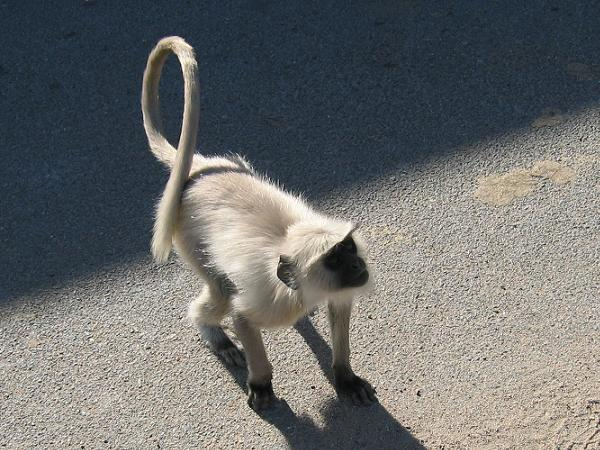
\includegraphics[width=5cm]{articles/La-vie-en-inde/singe.jpg}
\smallbreak

Allez les gens, à la prochaine.

\end{multicols}

\bigskip
\textbf{\textsc{Commentaires}}

\medskip
Peggy a écrit le 8 fév. 2008 :
\begin{displayquote}
C'est magique ton récit.
\end{displayquote}

\medskip
Titou a écrit le 8 fév. 2008 :
\begin{displayquote}
Toujours un grand plaisir de vous lire (au boulot) ! C'est vrai que ça a l'air d'être un univers complètement différent. J'ai beau être parti loin il n'y a rien de comparable. Faites gaffe à vous quand même avec les ti soucis sanitaires et surtout profitez toujours à fond de cette super expérience que vous êtes en train de vivre ! Merci de nous la faire partager. A très bientôt ! Biz à vous deux !
\end{displayquote}

\medskip
Poun's a écrit le 8 fév. 2008 :
\begin{displayquote}
C'est super de pouvoir partager un peu de votre expédition grâce aux commentaires et aux photos. Je pense qu'on est pas mal à attendre impatiemment le prochain épisode!
A bientôt.
\end{displayquote}

\medskip
Sam a écrit le 9 fév. 2008 :
\begin{displayquote}
Pfiou :) Je vous admire de mener une telle aventure ! Je ne pense pas pouvoir survivre à ça pendant plus de 48h.
En tout cas, vous voyez et vivez des choses magnifiques, c'est le principal ! Continuez à déjouer les arnaques et à vous en prendre plein la vue pour nous tous !
\end{displayquote}

\medskip
Les vadrouilleurs a écrit le 10 fév. 2008 :
\begin{displayquote}
Merci beaucoup pour vos messages, c'est vrai qu'on nous avait prévenu qu'on se prendrait une grosse claque en arrivant ici, et heureusement d'ailleurs car sinon\dots
\end{displayquote}

\medskip
Seb a écrit le 11 fév. 2008 :
\begin{displayquote}
Super sympa de nous faire partager tous ça, ça a l'air d'être super impréssionant là bas.
Bonne suite et que l'aventure continue.
\end{displayquote}

\medskip
Catherine a écrit le 11 fév. 2008 :
\begin{displayquote}
Vous me donnez de plus en plus envie de partir en Inde en juillet. Mais j'attends votre avis : est-ce profitable pour François et Marine ou faut-il attendre qu'ils soient plus agés ?
métier oblige : je suis sensible à la demande pour les écoliers et aimerais savoir ce qu'il est souhaitable d'envoyer et à quelle adresse ? (en recommandé où le facteur ne risque pas de se servir ?)
Vous nous transmettrez l'adresse à laquelle on vous enverra un peu d'argent quand les arnaques auront eu raison de votre porte-monnaie\dots
merci beaucoup à Cécile pour son appel.
\end{displayquote}

\medskip
La vadrouilleuse a écrit le 13 fév. 2008 :
\begin{displayquote}
Pour répondre au dernier commentaire, voici notre avis sur le fait d'emmener des enfants en vacances en Inde. On est catégoriques, d'apres notre expérience, non, les enfants restent à la maison. Trop de choses ici peuvent heurter leur sensibilité et les marquer à vie.
De même qu'une femme seule, ou meme deux jeunes femmes, ou une femme et ses enfants seront ici, on pense, sans arrêt regardés et il vaut mieux s'abstenir de voyager dans ces conditions. La condition de la femme n'est pas la même ici qu'en Europe.
\end{displayquote}

\medskip
Tatid a écrit le 21 fév. 2008 :
\begin{displayquote}
Je le disais dans un commentaire précédent (ou suivant plutôt puisque je lis le blog dans le sens non-chronologique :p), niveau confort et culture, ça doit faire un méga choc, surtout pour nous occidentaux qui avons besoin d'une certaine hygiène quoi\dots C'est vrai que je serais méfiant quant à la nourriture que je pourrais manger\dots
Sinon, vue comment vous décrivez ce qui se passe dans la rue, ça doit être un sacré bordel :-D Quant aux arnaques, je trouve ça abusé, profiter des touristes pour leur faire cracher de la thune tout le temps, grrr\dots
Félicitation quand même d'avoir eu le courage de vivre cette aventure (qui en est vraiment une en soi) !
Grâce à ce voyage, d'après ce que vous racontez, vous avez rencontré des gens assez exceptionnels, je pensais à Raj là, c'est génial ce qu'il fait pour les autres, ça doit être touchant de voir ces enfants pris en charge par un "grand enfant" qui veut leur apporter de la connaissance\dots J'ai hâte de voir les photos !
\end{displayquote}

\vfill

